\documentclass[11pt,a4paper]{article}

\usepackage{style2017}
\usepackage{hyperref}

\hypersetup{
    colorlinks =false,
    linkcolor=blue,
   linkbordercolor = 1 0 0
}
\newcounter{numexo}
\setcellgapes{1pt}

\begin{document}


\begin{Huge}Activité : Système d'exploitation GNU/linux \end{Huge}\medskip
\hrule
\vspace{1cm}

Le système d'exploitation GNU/Linux est un OS équivalent au système d'exploitation Windows. Il est gratuit et libre. Il dispose d'une interface graphique basée sur des fenêtres qui permettent d'afficher les contenus des dossiers et des fichiers. Il dispose de programmes pour réaliser des taches de base comme le traitement de texte ou l'affichage de photos.


\subsection*{-1-~Organisation du système de fichiers}

\begin{enumerate}
\item Comment sont organisés les fichiers dans l'OS GNU/Linux ?\vspace{2cm}

\item Comment se nomme et se note le dossier contenant tous les autres dossiers ? \vspace{1cm}

\item Quel est le dossier réservé aux utilisateurs ? Donner le chemin absolu de ce dossier.\vspace{1.5cm}

\item Comment se nomme votre dossier personnel ? Donner le chemin absolu de ce dossier.\vspace{1.5cm}

\end{enumerate}

\subsection*{-2-~Organiser ses fichiers et dossiers}

On considère l'arborescence de dossiers et fichiers suivante :

\begin{center}
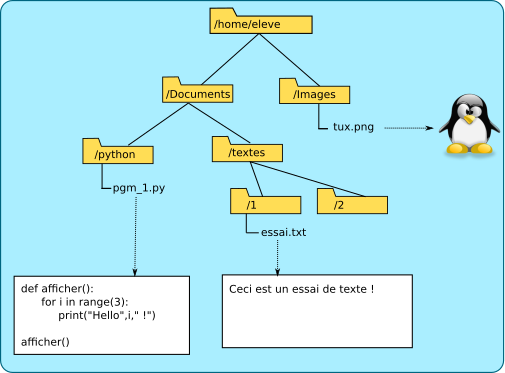
\includegraphics[scale=1]{../img/linux_dossier.png}
\end{center}

\newpage
\begin{enumerate}
\item Quels sont les dossiers déjà existant sur le système d'exploitation GNU/Linux? \vspace{2cm}

\item Créer les dossiers de l'arborescence qui manquent.

\item Ouvrir un éditeur de texte et créer le fichier \textsf{essai.txt}.

\item Pour écrire le programme Python, vous pouvez utiliser l'application \textsf{Thonny}. Saisir le programme puis l'enregistrer sous le nom \textsf{pgm\_1.py}.

\item Enregistrer l'image \textsf{tux.png} disponible sur la clé usb (la demander au prof!).

\item Donner les chemins absolus des 3 fichiers \textsf{essai.txt}, \textsf{pgm\_1.py} et \textsf{tux.png}. \vspace{2cm}
\end{enumerate}


\subsection*{-3-~Le terminal linux}

Linux peut être utilisé sans aucune interface graphique ce qui en fait sa force. L'utilisation de GNU/Linux se fait alors en ligne de commandes. Le \textsf{terminal} est une application qui permet de saisir des lignes de commandes.

\begin{enumerate}
\item  Ouvrir une nouvelle fenêtre de "Terminal". Ce terminal est aussi appelé console. Noter l'invite de commande proposée, c'est à dire tous les caractères situés avant le curseur de saisie!\vspace{1cm}

\item Il existe de très nombreuses commandes. On va en découvrir quelques unes assez simples mais très utiles que vous allez tester.

\begin{enumerate}
\item La commande \textsf{pwd} permet de savoir où l'on se trouve dans l'arborescence de fichiers. Dans quel dossier êtes-vous à l'ouverture du terminal ?\vspace{1cm}

\item La commande \textsf{ls} liste le contenu du dossier ou vous vous trouvez. Quels sont les dossiers et fichiers affichés  par cette commande ?\vspace{1cm} 

\item La commande \textsf{cd} permet de se déplacer dans l'arborescence. Elle doit être suivie du chemin absolu ou du chemin relatif vers le dossier que l'on souhaite atteindre. Pour remonter d'un niveau il faut saisir \textsf{..} !

Écrire les commandes puis les exécuter pour vous déplacer vers:\medskip
\begin{itemize}
\item le dossier \textsf{Images} : \medskip
\item le dossier \textsf{Documents}: \medskip
\item le dossier \textsf{python}: \medskip
\item le dossier \textsf{1}: \medskip
\item le dossier \textsf{eleve}: \medskip
\end{itemize}

\item La commande \textsf{mkdir} permet de créer un nouveau dossier. Il faut au préalable se placer dans le dossier qui contiendra le nouveau dossier. Puis on saisit la commande suivi du nom du dossier.\medskip

\begin{itemize}
\item Créer un dossier nommé \textsf{3} dans le dossier \textsf{Textes}. \medskip

\item Créer un dossier nommé \textsf{linux} dans le dossier \textsf{Images}. \medskip
\end{itemize}

\item La commande \textsf{mv} permet de déplacer un fichier d'un dossier à un autre. Elle est donc suivi du dossier contenant le fichier puis du dossier réceptionnant le fichier selon la syntaxe :

\textsf{mv /chemin/vers/fichier /chemin/nouveau/dossier}

\begin{itemize}
\item Déplacer le fichier texte \textsf{essai.txt} vers le dossier \textsf{3}. \medskip

\item Déplacer l'image \textsf{tux.png} vers le dossier \textsf{linux}. \medskip


\end{itemize}

\item La commande \textsf{tree} affiche l'arborescence du dossier où se trouve l'utilisateur. Afficher et reproduire l'arborescence du dossier \textsf{eleve}. \vspace{3cm}

\end{enumerate}



\end{enumerate}

\subsubsection*{-4-~La gestion des permissions}
Il y a trois types d'utilisateurs dans un système GNU/Linux:

\begin{itemize}
\item l'utilisateur \textsf{u} (user) qui est actuellement connecté et propriétaire de ces fichiers.
\item le groupe \textsf{g} (group) qui rassemble plusieurs utilisateurs.
\item les autres utilisateurs \textsf{o} (others).
\end{itemize}

Il y a trois types de permissions sur les dossiers et les fichiers dans GNU/Linux.

\begin{itemize}
\item Le droit en lecture : \textsf{r}
\item Le droit en écriture : \textsf{w}
\item Le droit en exécution : \textsf{x}
\end{itemize}

La commande \textsf{ls -l} affiche le contenu d'un dossier en donnant les permissions de chaque fichier et sous-dossier.

La figure ci-dessous donne un exemple de cet affichage:
\begin{center}
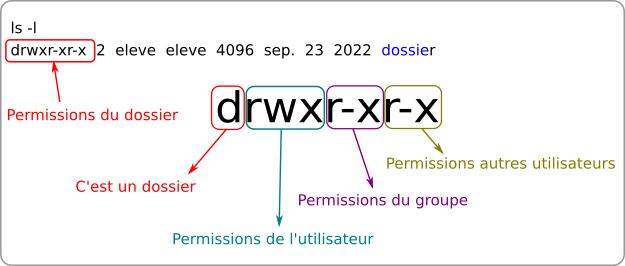
\includegraphics[scale=0.8]{../img/permission.png}
\end{center}

\begin{enumerate}
\item Lister le contenu du dossier \textsf{Documents} avec la commande \textsf{ls -l} puis relever les permissions du dossier \textsf{python} \vspace{1cm}

\item Lister le contenu du dossier \textsf{3} avec la commande \textsf{ls -l} puis relever les permissions du fichier \textsf{essai.txt} \vspace{1cm}



\newpage
\item La commande \textsf{chmod} modifie les permissions d'un dossier ou d'un fichier. La syntaxe est la suivante:

\begin{itemize}
\item \textsf{chmod g+w nom\_fichier} ajoute la permission \textsf{écrire} au groupe.
\item \textsf{chmod o-x nom\_dossier} enlève la permission \textsf{exécuter} aux autres utilisateurs.
\end{itemize}

\begin{enumerate}
\item Modifier les permissions d'un fichier.

\begin{itemize}
\item Enlever la permission de lecture au fichier \textsf{essai.txt} pour l'utilisateur propriétaire du fichier. Quelle est la commande à saisir ? \vspace{1cm}

\item Le fichier peut-il être affiché avec un éditeur de texte ? \vspace{1cm}

\item Remettre la permission sur le fichier \textsf{essai.txt} puis vérifier son édition.
\end{itemize}

\item Modifier les permissions d'un dossier.

\begin{itemize}
\item Enlever la permission d'\textsf{écriture} au dossier \textsf{2} pour l'utilisateur propriétaire du dossier. Quelle est la commande à saisir ? \vspace{1cm}

\item Déplacer le fichier \textsf{essai.txt} dans le dossier \textsf{2}. Que remarquez-vous ? \vspace{1cm}

\item Remettre la permission d'\textsf{écriture} au dossier \textsf{2} puis déplacer le \textsf{essai.txt} dans le dossier \textsf{2}.
\end{itemize}

\end{enumerate}


\end{enumerate}



\end{document}

